\documentclass[a4paper, 11pt]{article}
\usepackage[slovene]{babel}
\usepackage[utf8]{inputenc}
\usepackage[T1]{fontenc}
\usepackage{amsfonts,amsmath,amssymb}
\usepackage{amsthm}
\usepackage{amsmath}
\usepackage{amssymb}
\usepackage{graphicx}
\usepackage{relsize}
\usepackage{algpseudocode}  % za psevdokodo
\usepackage{algorithm}      % za
\usepackage[all]{xy}
\usepackage{changepage}

\floatname{algorithm}{Algoritem}
\renewcommand{\listalgorithmname}{Kazalo algoritmov}
\algnewcommand\algorithmicto{\textbf{to}}
\algnewcommand\algorithmicin{\textbf{in}}
\algnewcommand\algorithmicforeach{\textbf{for each}}
\algrenewtext{For}[3]{\algorithmicfor\ #1 $\gets$ #2\ \algorithmicto\ #3\ \algorithmicdo}
\algdef{S}[FOR]{ForEach}[2]{\algorithmicforeach\ #1\ \algorithmicin\ #2\ \algorithmicdo}


\theoremstyle{definition}
\newtheorem{definicija}{Definicija}
\theoremstyle{definition}
\newtheorem{opomba}{Opomba}
\newtheorem{izrek}{Izrek}
\newtheorem{trditev}{Trditev}
\newtheorem{lema}{Lema}
\newtheorem{primer}{Primer}

\newcommand{\G}{\mathcal{G}}
\newcommand{\E}{\mathcal{E}}
\newcommand{\V}{\mathcal{V}}

\begin{document}
    
\thispagestyle{empty}
\noindent{\large
UNIVERZA V LJUBLJANI\\[1mm]
FAKULTETA ZA MATEMATIKO IN FIZIKO\\[5mm]
FINANČNA MATEMATIKA  -- 1.stopnja}
\vfill

\begin{center}{\large
Matej Rojec, Vito Rozman, Ana Marija Belingar  \\[2mm]
{\textbf{Uravnotežen rdeče modri povezan podgraf} }\\[10mm]
Poročilo pri predmetu Finančni praktikum \\[1cm]}
\end{center}
\vfill

\noindent{\large
Ljubljana, 2022}

\newpage



    %\tableofcontents
    %\listoftables

    \tableofcontents
    \listoffigures
    \listoftables

    \newpage
    
    \section{Uvod}

    V poročilu bomo predstavili problem iskanja največjega povezanega 
    uravnoteženega podgrafa na mrežah velikosti $1 \times n$ (pot), $2\times n$, $3\times n$ in 
    $4\times n$, pri čemer je $n$ število stolpcev. Na začetku bomo predstavili 
    kako smo se lotili reševanja problema. Nato bomo predstavili kodo s 
    katero smo problem rešili, v zadnjem delu pa eksperimente, rezultate 
    in ugotovitve do katerih smo prišli. Za zaključek bomo navedli še 
    možne izboljšave.

    \section{Predstavitev problema}
        
    Naj bo $G = (V, E)$ graf. Vsako vozlišče $v \in V $ je obarvano rdeče ali modro. 
    Najti želimo največji povezani podgraf $G' = (V', E')$, ki ima enako število rdečih in modrih vozlišč.
    Velikost podgrafa je število njegovih vozlišč. Ta problem je v splošnem NP-težek, kar pomeni da ga ne moremo
    rešiti v polinomskem času.
    Osredotočili se bomo na optimalen algoritem za reševanje problema na mrežah oblike $1 \times n$ (pot), $2 \times n$, 
    $3 \times n$ in $4 \times n$.
    Naš algoritem je testiran na grafih, kjer so vožlišča obarvali rdeče z verjetnostjo $p \in (0,1)$ 
    in modro z verjetnostjo $1 - p$. 
    
    \section{Osnovni pojmi}
    
    \begin{definicija} (Induciran podgraf)
        Naj bo $G=(V,E)$ graf in naj bo $S \subseteq V$ podmnožica vozlišč grafa $G$. 
        Graf $G[S]$ je induciran podgraf grafa $G$, natanko takrat ko $\forall u, v \in S$ velja,
        da sta $u$ in $v$ sosednja v $G[S]$, natanko takrat ko sta sosednja v $G$.
    \end{definicija}
    
    V našem primeru bomo iskali največji povezan inducirani podgraf \\ $G' = (V', E')$ grafa $G = (V, E)$, kjer lahko možico volzlišč
    zapišemo kot: 
        $$ V' = V_{R} \cup V_{B},$$
    za katero velja $ V_{R} \cap  V_{B} = \emptyset $ in $|V_{R}| = |V_{B}| = \frac{|V'|}{2}$. Tako bomo dobili
    največji uravnotežen povezan podgraf z enakim številom rdečih in modrih vozlišč.    

    \begin{definicija} (Pot) Graf $P_n=(V,E)$ je pot, kjer je
        $V=\{ v_1,...,v_n \}$, če je množica povezav oblike:
        $E = \{ (1, 2),(2, 3),...,(n-1, n) \}$.
    \end{definicija}

    \begin{definicija} 
    (Mreža) Graf $M_{m,n}=(V,E)$ je mreža velikosti $m \times n$, 
    kjer je $V=\{ v_{1,1},...,v_{1,n},v_{2,1},...,v_{2,n},...,v_{m,1},...,v_{m,n} \}$, če je množica povezav oblike:
        $$
        E = \{ ((i, i'),(j, j')) \mid |i-i'| + |j-j'| =1  \}
        $$
    \end{definicija}

    \begin{definicija}
    (Particija vzorcev)  
    Naj bo $G$ graf. 
    Za graf $G \square P_{n-1}$ je $\mathcal{V}$ particija množice povezanih komponent podgrafa grafa $G$.  
    \end{definicija}

    \begin{definicija}
    (Združljiva vzorca) 
    Vzorca $u$ in $v$ sta združljiva, pišemo \newline $u \sim v$, če ko pogledamo unijo
    induciranih podgrafov grafa $G$ na vozliščih iz $u$ 
    oziroma $v$, potem za vsako povezano komponento v istem delu $v$ velja, da pripada isti povezani komponenti v uniji (pri čemer upoštevamo povezanost komponent v istem delu $u$).   
    \end{definicija}


\section{Algoritem}
    Ogledali si bomo problem na mrežah ($ m \times n$), pri čemer bomo uporabili
    dinamično programiranje. Algoritem sprejme kot vhod mrežo $m \times n$, 
    kjer je vsako vozlišče obarvano bodisi modro bodisi rdeče. 

    \vline

    Definirajmo spremenljivke:
    \begin{itemize}
        \item 
        $x_{ik} = 1$, če je $k$-to vozlišče v $i$-tem stolpcu rdeče, in $-1$, če je modro
        \item 
        $p_{ijv}$ je velikost največji podgraf do $i$-tega stolpca z razliko $j$, kjer je v zadnjem stolpcu uporabljeni vzorec $v$   
        \item 
        $\mathcal{V}_{ijv}$  so vozlišča največjega podgrafa do $i-$tega stolpca z razliko $j$, kjer
        je v zadnjem stolpcu uporabljen vzorec $v$
    \end{itemize}

    Začetni pogoji so:
    \begin{itemize}
        \item 
        $p_{10v} = 0$
        \item
        $ p_{1jv} =
            \begin{cases}
            |v|, & \text{če}\ j = \sum_{k \in v}x_{1k} \\
            -\infty, & \text{če}\ j \ne \sum_{k \in v}x_{1k} \quad$ in $\quad j\ne 0
            \end{cases}
        $
        \item 
        $p_{ijv} = -\infty$, če je $\quad |j| > i |G|$ 
    \end{itemize}

    Rekurzivne enačbe:
    $$
    p_{ijv} = |v| ~+~ \max\left(\{p_{i-1, j - \sum_{k \in v} x_{ik}, u} \mid u \sim v\} \cup \{-|v| \mid j = 0\}\right) ,\ (-i|G| \le j \le i|G|) 
    $$
    
    Optimalna rešitev:
    $$p^* = \max\{p_{i0v} \mid i \le 1 \le n, v \text{ povezan}\}$$



Na vsakem koraku algoritma izračunamo $p_{ijv}= |v| + \eta$ ter najdemo pripadajočo množico $\mathcal{V}_{ijv}$.
Množico $\mathcal{V}_{ijv}$, če ta ni prazna, dobimo tako, da ji dodamo vozlišča vzorca $v$ in množico
vozlišč, kjer je dosežena $\eta$.

    
Za programerski del naloge smo uporabljali Python. V nadaljevanju so predstavljenje glavne funkcije, 
ki smo jih za ta del definirali.

Glavni funkciji se nahajata v \verb+algoritem.py+, ki 
sta \verb+P+, ki izračuna vse vsrednosti $p_{ijv}$ od zgoraj ter 
pripdajoč graf ter \verb+max_BCS+, ki najde največji
uravnotežen povezan podgraf.  

Pomožna datoteka \verb+modelBCS.py+ vsebuje razred
\verb+BSC+, ki generira osnovne parametre za lažji izračun.
\newpage

\section{Eksperimenti}

V tem delu seminarske naloge smo se ukvarjali s tremi ključnimi vprašanji:
    
\begin{itemize}
\item 
Kako se velikost rešitve spreminja glede na verjetnost $p$.
\item
Kako se velikost rešitve spreminja glede na dolžino mreže $n$.
\item 
Kako se hitrost algoritma spreminja, če večamo $n$ in $m$.
\end{itemize}

\subsection{Delež vozlišč v BCS grafu glede na verjetnost $p$} 

Za odgovor na prvo vprašanje smo za $m=1$ in $m=2$ izvedli 500 ponovitev 
poskusa ter za $m=3$ in $m=4$ pa 250 ponovitev poskusa na mreži dolžine $n=50$ pri različnih verjetnostih. 
Slika \ref{fig:verj} prikazuje rezultate.

\begin{figure}[ht!]
    \centering
    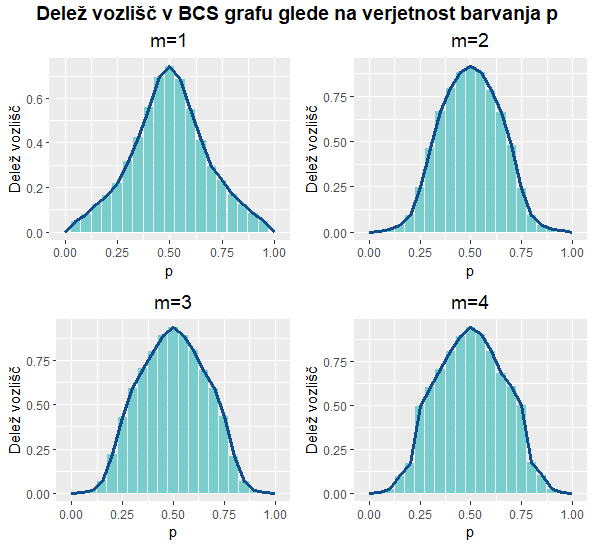
\includegraphics[width=0.75\textwidth]{verj.png}
    \caption{Prikaz porazdelitve za $n=50$ ter $m \in \{ 1,2,3,4 \}$.}
    \label{fig:verj}
\end{figure}

Prva ugotovitev je, da je za posamezen $m$  največja rešitev pri $p=0.5$, 
kar je pričakovano, saj je takrat število modrih in rdečih vozlišč v 
grafu v povprečju enako, zato je verjetnost da dobimo uravnotežen povezan 
podgraf največja. 
Bolj kot se bližamo robovom ($p=0$ ali $p=1$), manjšo rešitev dobimo. 
Iz eksperimentov se zdi 
, da se z dodajanjem vrstic (večanjem $m$-ja) veča tudi delež vozlišč glede 
na velikost celotnega grafa pri fiksnem $p$.

\newpage

\subsection{Delež vozlišč v BCS grafu glede na velikost mreže}

Za odgovor na drugo vprašanje smo za vsak $m$ posebej izvedli 250 ponovitev pri 
verjetnosti barvanja grafa $p = 0.5$ in pri različnih dolžinah grafa 
(tj. različnih $n$-jih). 

\begin{figure}[h]
    \centering
    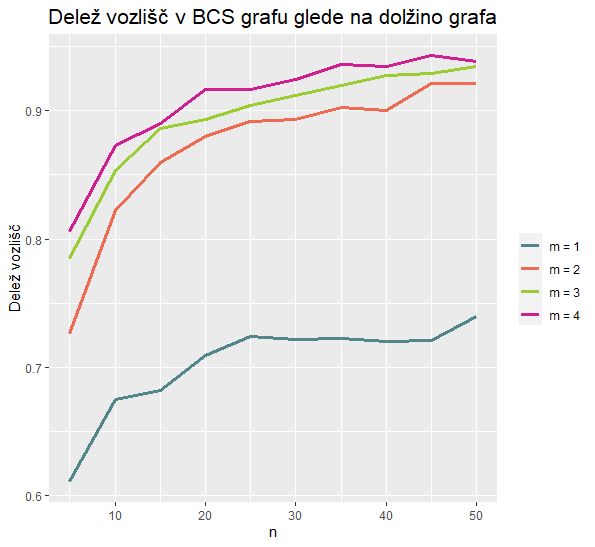
\includegraphics[width=0.75\textwidth]{delez.png}
    \caption{Prikaz deleža vozlišč v grafu pri $p=0.5$ v
    odvisnosti od $n$.}
    \label{fig:delez}
\end{figure}


Kot vidimo iz slike \ref{fig:delez} je delež vozlišč glede na 
velikost celotne poti veliko manjši kot pri ostalih $m$-jih. 
Iz grafa vidimo, da ne gre za linearno rast, ampak morda za logaritmično.


\subsection{Hitrost BSC glede na velikost mreže}

Kot zadnji eksperiment smo raziskovali časovno zahtevnost našega algoritma kar je 
razvidno iz slike \ref{fig:cas} ter tabele \ref{tab:cas}.
Podatki prikazujejo povprečen čas izvajanja algoritma v sekundah. 


\begin{figure}[h]
    \centering
    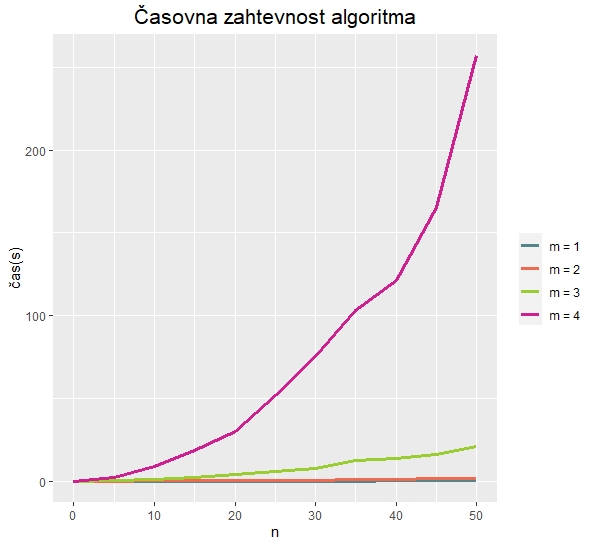
\includegraphics[width=0.75\textwidth]{cas.png}
    \caption{Prikaz deleža vozlišč v grafu pri $p=0.5$ v
    odvisnosti od $n$.}
    \label{fig:cas}
\end{figure}

\begin{table}[!ht]
    \caption{Tabelirane vrednosti}
    \label{tab:cas}
    \begin{adjustwidth}{-2cm}{}
    \begin{tabular}{|l|l|l|l|l|l|l|l|l|l|l|l|}
    \hline
        $m$ $\backslash$ $n$ & 0 & 5 & 10 & 15 & 20 & 25 & 30 & 35 & 40 & 45 & 50 \\ \hline
        1 & 0.000 & 0.003 & 0.012 & 0.039 & 0.074 & 0.083 & 0.107 & 0.119 & 0.132 & 0.147 & 0.158 \\ \hline
        2 & 0.000 & 0.035 & 0.127 & 0.209 & 0.301 & 0.481 & 0.691 & 0.903 & 1.215 & 1.527 & 1.859 \\ \hline
        3 & 0.000 & 0.286 & 1.046 & 2.260 & 3.968 & 5.861 & 7.481 & 12.710 & 13.544 & 16.206 & 20.785 \\ \hline
        4 & 0.000 & 2.309 & 9.090 & 18.551 & 30.035 & 51.521 & 75.599 & 103.006 & 121.200 & 165.482 & 257.030 \\ \hline
    \end{tabular}
    \end{adjustwidth}
\end{table}

Iz grafa \ref{fig:cas} je razvidno, da je algoritem bistveno počasnejši za 
velike $n$.

\section{Zaključek}

Iz analize rezultatov lahko zaključimo, da imajo mreže največji 
uravnotežen rdeče modri povezan podgraf pri $p=0.5$, kar smo tudi
pričakovali. Zanimivo nam je bilo, kako se delež vozlišč v BCS 
grafu pri $m=1$ v odvisnosti od $p$ razlikuje od ostalih $m$-jev.
Za $p$ blizu $0.5$ je delež pri večjih $m-$jih večji, medtem ko je za 
$p \in \{ 0,1 \}$ ta delež večji pri $m=1$.
Vredno je omeniti, da mreže ne vsebujejo enako vozlišč in 
zato je morda rezultat (delež vzorcev) bolj natančen za večji $m$.
Iz naslednje analize lahko opazimo, da $m=1$ izstopa, saj 
ima nekoliko manjši delež vozlišč v primerjavi z drugimi.
Iz zadnje anlize pa vidimo, da za večje $m$ algoritem porabi bistveno
več časa kot za manjše, kar je posledica velikega števila vzorcev,
ki jih mora pregledati ter ostalih računskih operacij.  


\end{document}  
